\documentclass{article}
\usepackage[utf8]{inputenc}
\usepackage[letterpaper, margin=1.5in]{geometry}

\usepackage{setspace}
\doublespacing
\usepackage{graphicx}
\graphicspath{ {./images/} }
\usepackage[
backend=biber,
style=alphabetic,
sorting=ynt
]{biblatex}
\usepackage{gb4e}

\usepackage{multicol}
\setlength{\columnsep}{1cm}

\addbibresource{refs.bib}

\usepackage{tipa}

\title{A Phonetic Analysis of Norwegian}
\author{Derek Andersen}
\date{August 2020}

\begin{document}

\maketitle

\section{Introduction}
Norwegian is a North Germanic language spoken mainly in Norway, although it's also spoken in other countries such as Denmark, Sweden, and Germany. Norwegian has two official literary varieties: \textit{Nynorsk} (``new Norwegian") and \textit{Bokmål} (``book language"). The emergence of these two varieties was during Norway's separation from Denmark in 1814. This paper will be focusing on both varieties of Norwegian, however, as they are mutually intelligible with only slight variations. Importantly, both varieties share the same consonants and vowels. \cite{Omniglot}  

In this paper, I will provide a phonetic analysis of Norwegian. In Sections 2 and 3, I will outline the consonant and vowel inventories (respectively) of Norwegian and discuss the distribution of sounds and how they vary from those of English. In Section 4, I will give an analysis of the syllable structure of Norwegian words. In Section 5, I will discuss some allophonic rules that the phonemes of Norwegian undergo, and in Section 6, I will outline the stress patterns and prosody rules observed in Norwegian utterances.

\section{Consonant Inventory}
In comparison to English, the consonant inventory of Norwegian varies to a significant degree. Specifically, there are some sounds in English which are absent in Norwegian (notably the interdental fricatives \textipa{/\texttheta/ and /\dh/, the labio-velar approximant /w/, the voiced fricatives /v/ and /z/, and the palatoalveolar affricates /\textteshlig/ and /\textdyoghlig/}), and there are several sounds in Norwegian that don't exist in English (notably the labiodental approximant \textipa{/\textscriptv/, the alveolar trill /r/, the retroflex stops /\textrtailt/ and /\textrtaild/, the retroflex fricative /\textrtails/, the retroflex lateral approximant /\textrtaill/, the retroflex nasal /\textrtailn/, and the palatal fricative /\c{c}/}). \cite{LearnNorwegian} Noteworthy is the lack of affricate consonants entirely in Norwegian. A full IPA consonant chart for Norwegian is shown in Figure \ref{ConsChart}.

\begin{figure}[h]
    \centering
    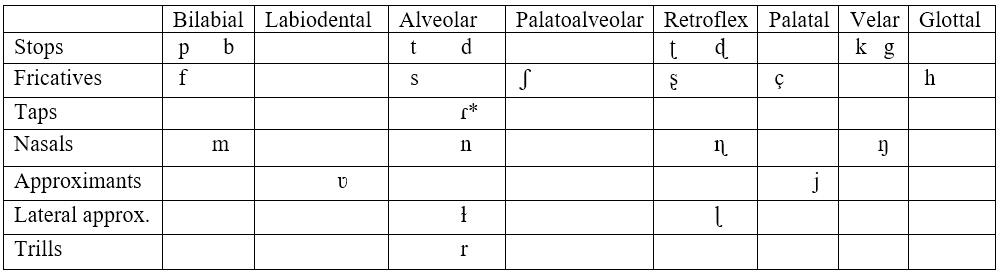
\includegraphics[scale=.55]{images/consonants.PNG}
    \caption{Norwegian consonant chart (IPA)}
    \label{ConsChart}
\end{figure}

* According to some sources, the alveolar trill /r/ is actually an alveolar tap /\textfishhookr/. \cite{TheGermanicLanguages}

\subsection{Minimal pairs}
To illustrate that these consonants are indeed separate phonemes and thus contrastive, I provide a few minimal (and near-minimal) pairs in \ref{MinPairCons}. \cite{RhinoSpike}, \cite{Norwegian101}

\begin{exe}
    \ex
    \label{MinPairCons}
    \begin{multicols}{2}
    \begin{itemize}
        \item [a.] \textit{sjelen} \textipa{/\textesh e\textrtaill en/} `soul' (n.)
        \item [] \textit{kjelen} \textipa{/\c{c}e\textrtaill en/} `boiler' (n.)
        \item [b.] \textit{skjære} \textipa{/\textesh\ae re/} `cut' (v.)
        \item [] \textit{kjære} \textipa{/\c{c}\ae re/} `dear' (adj.)
        \item [c.] \textit{gjenta} \textipa{/gjenta/} `repeat' (v.)
        \item [] \textit{jenta} \textipa{/jenta/} `girl' (n.)\columnbreak
        \item [d.] \textit{det} \textipa{/de/} `the' (art.)
        \item [] \textit{let} \textipa{/\textrtaill et/} `look' (v.)
        \item [e.] \textit{kan} \textipa{/kan/} `can' (v.)
        \item [] \textit{ran} \textipa{/ran/} `robbery' (n.)
    \end{itemize}
    \end{multicols}
\end{exe}

\section{Vowel Inventory}

The monophthong vowels of Norwegian do overlap a bit with those of English, but not unlike the consonant inventory, there are some vowels which exist only in Norwegian, and some which exist only in English. Specifically, both the high and the mid front rounded vowels /y/ and /ø/ and the high central rounded vowel /\textbaru/ are only present in Norwegian. A full IPA monophthong vowel chart for Norwegian is shown in Figure \ref{VowelChart}. \cite{TheGermanicLanguages}
\begin{figure}[h]
    \centering
    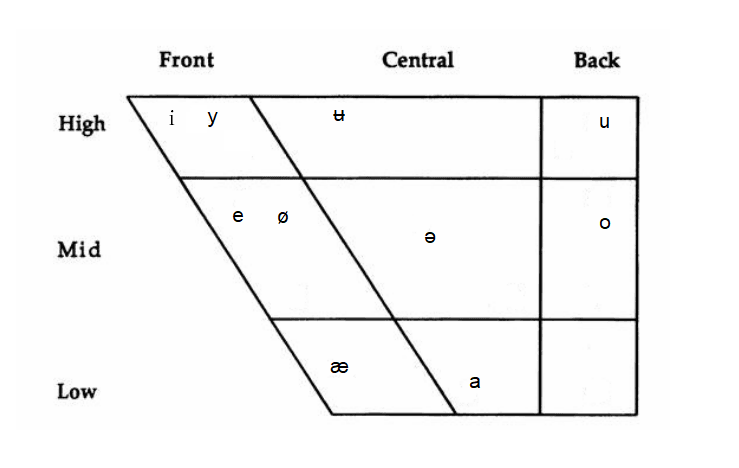
\includegraphics[scale=.6]{images/vowels.PNG}
    \caption{Norwegian monophthong chart (IPA)}
    \label{VowelChart}
\end{figure}

/æ/ is phonemic in Norwegian, but it also acts as an allophone of /e/, in the environment of ``preceding /r/". [\textschwa] is not phonemic, and considered an allophone of /e/. \cite{TheGermanicLanguages}

Norwegian also uses five diphthong vowels, some of which are (almost) present in English. Several different sources list the Norwegian diphthong inventory differently, but the most consistent inventory is the following: /ei/, /oi/, /ai/, /øy/, and /a\textbaru/. \cite{TheGermanicLanguages} While the first three are very close to English /e\textsci/, /\textopeno\textsci/, and /a\textsci/ respectively, a native English speaker could benefit from some example words which contain vowels resembling (but not identical to) the last two diphthongs. The vowel in the word `gooey' is close to /øy/, and the vowel in the word `mouse' is close to /a\textbaru/. \newline \newline
A vowel chart illustrating the path of the vowel quality change for the Norwegian diphthongs is shown in Figure \ref{DiphChart}.

\begin{figure}[h]
    \centering
    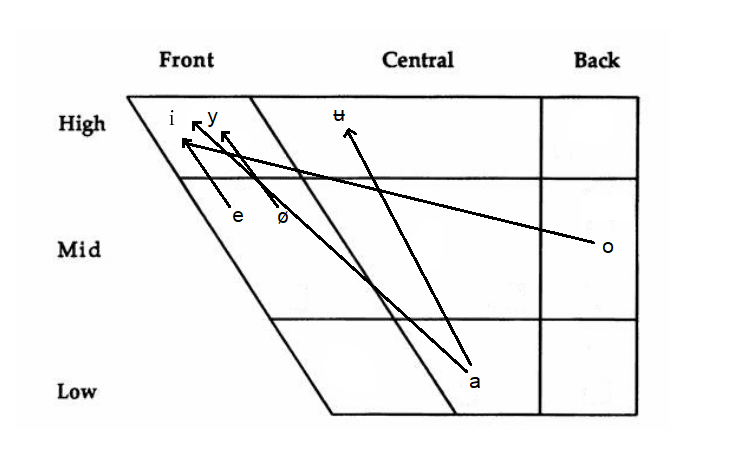
\includegraphics[scale=.6]{images/diph.PNG}
    \caption{Norwegian diphthong path chart (IPA)}
    \label{DiphChart}
\end{figure}

\subsection{Minimal pairs}
To illustrate that these vowels are indeed separate phonemes and thus contrastive, I provide a few minimal pairs in \ref{MinPairVowel}. \cite{RhinoSpike}, \cite{Norwegian101}

\begin{exe}
    \ex
    \label{MinPairVowel}
    \begin{multicols}{2}
    \begin{itemize}
        \item [a.] \textit{låven} \textipa{/\textrtaill oven/} `barn' (n.)
        \item [] \textit{loven} \textipa{/\textrtaill uven/} `law' (n.)
        \item [b.] \textit{vi} \textipa{/vi/} `we' (pro.)
        \item [] \textit{ve} \textipa{/ve/} `woe' (n.)
        \item [c.] \textit{gjøre} \textipa{/gjør\textschwa/} `do' (v.)
        \item [] \textit{gjare} \textipa{/gjar\textschwa/} `make' (v.)\columnbreak
        \item [d.] \textit{nei} \textipa{/nai/} `no' (n.)
        \item [] \textit{nøy} \textipa{/nøy/} `settle' (v.)
        \item [e.] \textit{sa} \textipa{/sa/} `so' (adv.)
        \item [] \textit{sau} \textipa{/sa\textbaru/} `sheep' (n.)
        
    \end{itemize}
    \end{multicols}
\end{exe}


\section{Syllable Structure}

The syllable structure of Norwegian is fairly unrestrictive, and allows for a wide range of allowed configurations of consonant clusters in both onset and coda. Both complex onsets and complex codas are allowed, but onsets are codas aren't always present. Specifically, the constraints allow for a syllable structure as bare as a lone V in the nucleus, or one as rich as a V padded by clusters of as many as three consonants (CCC) in both onset and coda. All allowed structures, according to sources which list them explicitly, are listed in \ref{CV}. \cite{TheGermanicLanguages}

Notably, however, in my research I wasn't able to find a word or syllable which follows the CCCVCCC structure (the maximal example being CCVCCC /b\textrtaill omst/ listed in \ref{cv2}c). Possibly, the fact that Norwegian is an agglutinative language (which allows for morphemes to be ``stuck on" to each other quite freely to construct new words) might be the reason for CCCVCCC being an acceptable syllable structure, although it doesn't seem to show up in more frequently used words.

\begin{exe}
    \ex
    \label{CV}
    \begin{multicols}{3}
    
    \begin{itemize}
        \item [] V
        \item [] CV
        \item [] VC
        \item [] CCV
        \item [] VCC
        \item [] CCCV
        \item [] VCCC
        \item [] CVC
        \item [] CCVC
        \item [] CCCVC
        \item [] CVCC
        \item [] CVCCC
        \item [] CCVCC
        \item [] CCCVCC
        \item [] CCVCCC
        \item [] CCCVCCC
    \end{itemize}
    
    \end{multicols}
\end{exe}

A few examples of three-consonant onset clusters are shown in \ref{cv1}, and examples of three-consonant coda clusters are shown in \ref{cv2}. \cite{TheGermanicLanguages}

\begin{exe}
    \ex
    \label{cv1}
    \begin{itemize}
        \item [a.] \textit{språk} /sprok/ `language' (n.)
        \item [b.] \textit{strøm} /strøm/ `current' (n.)
        \item [c.] \textit{skrue} /skr\textbaru\textschwa/ `screw' (n.)
    \end{itemize}
\end{exe}
\newpage
\begin{exe}
    \ex
    \label{cv2}
    \begin{itemize}
        \item [a.] \textit{hatsk} /hatsk/ `hateful' (adj.)
        \item [b.] \textit{vekst} /vekst/ `growth' (n.)
        \item [c.] \textit{blomst} /b\textrtaill omst/ `flower' (n.)
    \end{itemize}
\end{exe}

In Figure \ref{blomst}, I provide a syllable structure tree for example \ref{cv2}c /b\textrtaill omst/. This word follows the CCVCCC structure.

\begin{figure}[h]
    \centering
    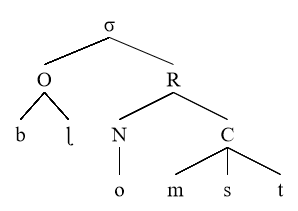
\includegraphics[scale=.6]{images/blomst.PNG}
    \caption{Syllable structure tree for /b\textrtaill omst/}
    \label{blomst}
\end{figure}

The constraints which govern the particular consonants which are allowed in onset and coda seem to be quite similar to those of English. For example, Norwegian has a word \textit{angst} \textipa{/a\ng st/} `anxiety' (n.), which has a CCC coda \textipa{/\ng st/}. This sequence is acceptable in codas, but doesn't appear in onsets — just like English. Similarly, the word \textit{valp} \textipa{/va\textrtaill p/} `puppy' (n.) has a CC coda \textipa{/\textrtaill p/}. This sequence is acceptable in codas, but doesn't appear in onsets (like /lp/ in English).

\section{Allophonic Rules}
\subsection{Palatalization of alveolar consonants}
The alveolar consonants in Norwegian, namely /t/, /d/, /n/, /s/, and /\textltilde/, are known to undergo palatalization in stressed syllables, or even in both stressed and unstressed syllables in some dialects. \cite{Wikipedia} The phoneme to allophone conversions for this palatalization are outlined in \ref{palatal}. While I was unable to find an example of this process in my research, the assumption is that when the alveolar consonant is at the beginning of the onset of a stressed syllable, palatalization occurs, like in the hypothetical example in \ref{hypo}.

\begin{exe}
    \ex
    \label{palatal}
    \begin{multicols}{2}
    \begin{itemize}
        \item [] /t/ $\rightarrow$ [c]
        \item [] /d/ $\rightarrow$ [\textObardotlessj]
        \item [] /n/ $\rightarrow$ [\textltailn]
        \item [] /s/ $\rightarrow$ [\c{c}]
        \item [] /\textltilde/ $\rightarrow$ [\textturny]
    \end{itemize}
    \end{multicols}
\end{exe}

\begin{exe}
    \ex
    \label{hypo}
    \textit{tomt} `empty' (adj.)\newline /tomt/ $\rightarrow$ [comt] (palatalization of /t/)
\end{exe}

\subsection{Reduction of /e/ $\rightarrow$ /\textschwa/}
As I briefly mentioned in Section 3, [\textschwa] is not phonemic in Norwegian. Instead, it acts as an allophone of /e/. Based on a few examples I've seen during my research, like the one in \ref{schwa}, the process seems to be ``/e/ becomes /\textschwa/ in unstressed syllables." In this example, the word-final /e/ is unstressed, and thus its reduction to /\textschwa/ is licensed. 

\begin{exe}
    \ex
    \label{schwa}
    \textit{skrue} `screw' (n.) \newline /\textprimstress skr\textbaru e/ $\rightarrow$ [\textprimstress skr\textbaru\textschwa] (reduction of /e/)
\end{exe}

\subsection{/e/-lowering}
The vowel /\textipa{\ae}/, while phonemic in Norwegian, is also seen as an allophone of /e/ in the environment of ``preceding /r/". \cite{TheGermanicLanguages} An example of this process is shown in \ref{lowering}. \cite{Norwegian101}

\begin{exe}
    \ex
    \label{lowering}
    \textit{er} `is' (v.)\newline /er/ $\rightarrow$ [\textipa{\ae}r] (lowering of /e/)
\end{exe}

\section{Stress and Prosody}
\subsection{Word-level stress}
As a general rule, word-level stress in Norwegian most of the time falls on the first syllable of a word, if the word is polysyllabic. This is shown in the examples in \ref{first}. \cite{TransparentLanguage}

\begin{exe}
    \ex
    \label{first}
    \begin{itemize}
        \item [a.] \textit{sola} /\textprimstress su\textrtaill a/ `sun' (n.)
        \item [b.] \textit{skrue} /\textprimstress skr\textbaru\textschwa/ `screw' (n.)
    \end{itemize}
\end{exe}

An exception to this rule is the prefixation of some words of Norwegian, for example, in \textit{be-} and \textit{for-} prefixation (among others). In these cases, the prefix signals stress to occur on the second syllable. Some examples of this process are shown in \ref{second}. \cite{TransparentLanguage}

\begin{exe}
    \ex
    \label{second}
    \begin{itemize}
        \item [a.] \textit{betaling} \textipa{/b\textschwa \textprimstress ta\textrtaill i\ng/} `payment' (n.)
        \item [b.] \textit{foreldre} \textipa{/fø\textprimstress re\textrtaill dr\textschwa/} `parents' (n.)
    \end{itemize}
\end{exe}

Another exception to the general rule is in the case of foreign loanwords, for which the stress is placed on the ultimate or penultimate syllable, depending on the number of syllables in the word. Examples of this process are shown in \ref{penult}. \cite{TransparentLanguage}

\begin{exe}
    \ex
    \label{penult}
    \begin{itemize}
        \item [a.] \textit{sjokolade} \textipa{/\textesh oko\textprimstress \textrtaill ad\textschwa/} `chocolate' (n.)
        \item [b.] \textit{mineral} \textipa{/min\textschwa\textprimstress ra\textltilde/} `mineral' (n.)
    \end{itemize}
\end{exe}

\subsection{Phrasal stress}
Although there are likely exceptions to this general pattern, in my research, I found that phrasal stress is assigned similarly to that of English — that is, the right-most content word is assigned the strongest phrasal stress, and a general pattern of alternation between the remaining words is followed for phrasal stress assignment. Importantly, function words are not candidates for phrasal stress, such as in the example in \ref{phrase}, taken from \cite{TransparentLanguage}. The function words are italicized, and stress has been assigned to the remaining words. Interestingly, the Norwegian and English word order (at least for this particular sentence) and stress assignment under my analysis are identical, possibly suggesting a correlation between word order and phrasal stress assignment.

\begin{exe}
    \ex
    \label{phrase}
    \begin{itemize}
        Jeg l\'iker \textit{å} pr\'ate \textit{med} \'Ola \textit{og} K\textdoublevbaraccent{a}ri.\newline `I l\'ike \textit{to} t\'alk \textit{with} \'Ola \textit{and} K\textdoublevbaraccent{a}ri.'
    \end{itemize}
\end{exe}

\section{Conclusion}
In this paper, I discussed the phonetic inventory of Norwegian, including consonants and vowels, and at times drew parallels to English when applicable. I also discussed the phonetic rules which govern how certain sounds are realized in speech.  

Based on my analyses, I believe that a hypothetical Norwegian learner would be well-equipped to learn English, and vice versa. In particular, while the consonant inventory of English and Norwegian vary significantly, there exist very few foreign manners and places of articulation in the overlap between both languages. For example, the only manner of articulation which would be foreign and thus difficult to a Norwegian speaker learning English would be affricates, and the only place of articulation which would be foreign and thus difficult to an English speaker learning Norwegian would be palatal (ignoring English /j/).  

The same goes for the vowels present in only one of the two languages. Vowels exist in both languages at each point in the vowel space, using a vowel chart as reference. A good understanding of the vowel space, tenseness, and lip rounding is all that's required to learn these foreign vowels. For these reasons, and given the fact that there are several other similarities between both languages, I feel that the only barrier to learning the foreign sounds would be the time required to practice producing these new sounds.


\printbibliography

\end{document}
